\documentclass[12pt, a4paper, oneside]{article}
\usepackage{graphicx}
\usepackage{arial}
\renewcommand{\familydefault}{\sfdefault}
\usepackage[T1]{fontenc}
\usepackage[polish]{babel}
\usepackage[utf8]{inputenc}
\usepackage{lmodern}
\usepackage[left=2cm,right=2cm,top=2cm,bottom=2cm]{geometry}
\selectlanguage{polish}

\begin{document}
\pagenumbering{arabic}
\section{Wstęp}
W DPCM - Differential Pulse Coded Modulation, przy niewielkiej szybkości zmian amplitudy sygnału źródłowego, rozważamy kodowanie jedynie przyrostów pomiędzy próbkami. Pozwala to uniknąć kodowania nadmiernej informacji w postaci składowej stałej. Prowadzi to do redukcji bitowej reprezentacji. Podstawowym przykładem realizacji DPCM jest Modulacja Delta (DM). W klasycznej DM problem stanowi jednak dobranie optymalnej wartości $\Delta$.
\subsection{ADM - Adaptive Delta Modulation}
Problem ten został rozwiązany w ADM poprzez adaptacyjną zmianę parametru $\Delta$. Istnieje wiele reguł aktualizacji delty, jednak najpopularniejszą z nich jest poniższa formuła:
\begin{equation}
\Delta(n)=\Delta(n-1)\cdot K^{e_{wy}(n)\cdot e_{wy}(n-1)},~\Delta(0)\geq0,~K>1
\end{equation}
W przypadku zbyt szybko narastającego lub zbyt szybko malejącego zbocza $\Delta$ zostaje zwiększona, a~przy sygnale wolnozmiennym - zmniejszona. Pozwala to na ciągłe dopasowywanie się do sygnału. Przy zbyt dużych wartościach parametru K może dojść do powstania szumu śrutowego. Odpowiedni dobór $\Delta$(0) oraz K jest tematem tego laboratorium.
\subsection{ADPCM - Adaptive Differential Pulse Coded Modulation}
W celu zwiększenia efektywności działania układu ADM zaproponowano wykorzystanie filtra adaptacyjnego zbudowanego na strukturze stabilnej w sensie BIBO - filtr FIR. W praktyce kodery ADPCM to predykcyjne filtry cyfrowe składające z~części statycznej - filtra IIR oraz adaptacyjnej - filtra FIR. W~uproszczonej analizie opisywany jest jedynie część adaptacyjna. ADPCM cechuje się następującą złożonością obliczeniową:
\begin{equation}
R=f_s(3p+1)=f_s\cdot K,
\end{equation}
gdzie:
\begin{itemize}
\item R - ilość mnożeń wykonywanych w ciągu sekundy,
\item K - ilość mnożeń elementarnych,
\item f$_s$ - częstotliwość próbkowania,
\item p - długość filtru.
\end{itemize}
\begin{figure}[h]
\centering
\caption{Schemat kodera ADPCM z 4 - bitowym kwantyzerem dynamicznym}
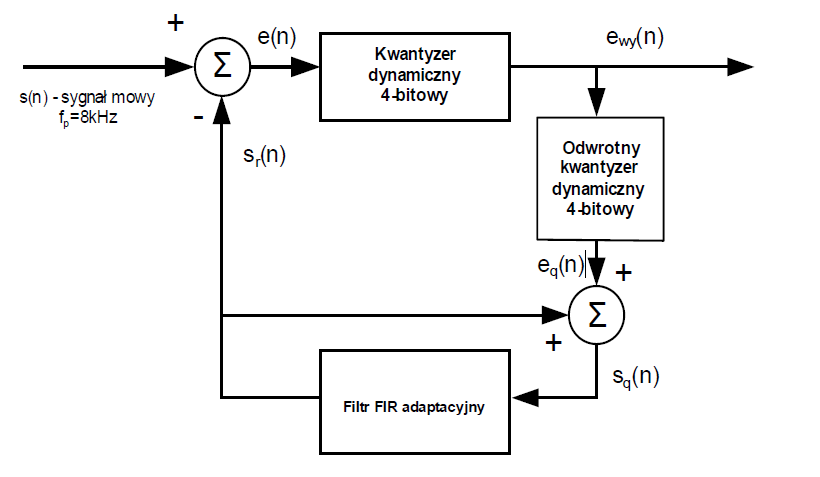
\includegraphics[scale=0.46]{f1.png}
\end{figure}
\clearpage
\section{Wyznaczanie optymalnych wartości parametrów $\Delta$ oraz K}
\subsection{Wyznaczenie optymalnej wartości $\Delta$(0)}
\begin{figure}[h]
\centering
\caption{Wykres $\Delta$(n) dla K = 1.01}
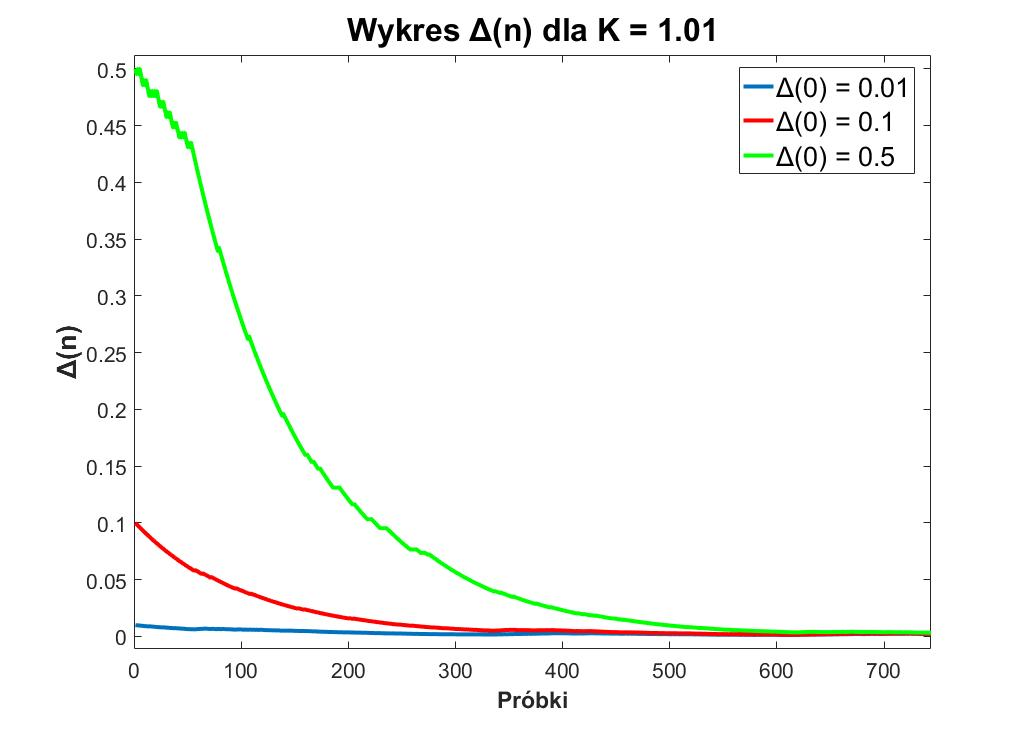
\includegraphics[scale=0.33]{f1.jpg}
\end{figure}
\begin{center}
Okres przejściowy T$_p$ = 600 próbek
\end{center}
\begin{figure}[h]
\centering
\caption{Wykres $\Delta$(n) dla K = 1.1}
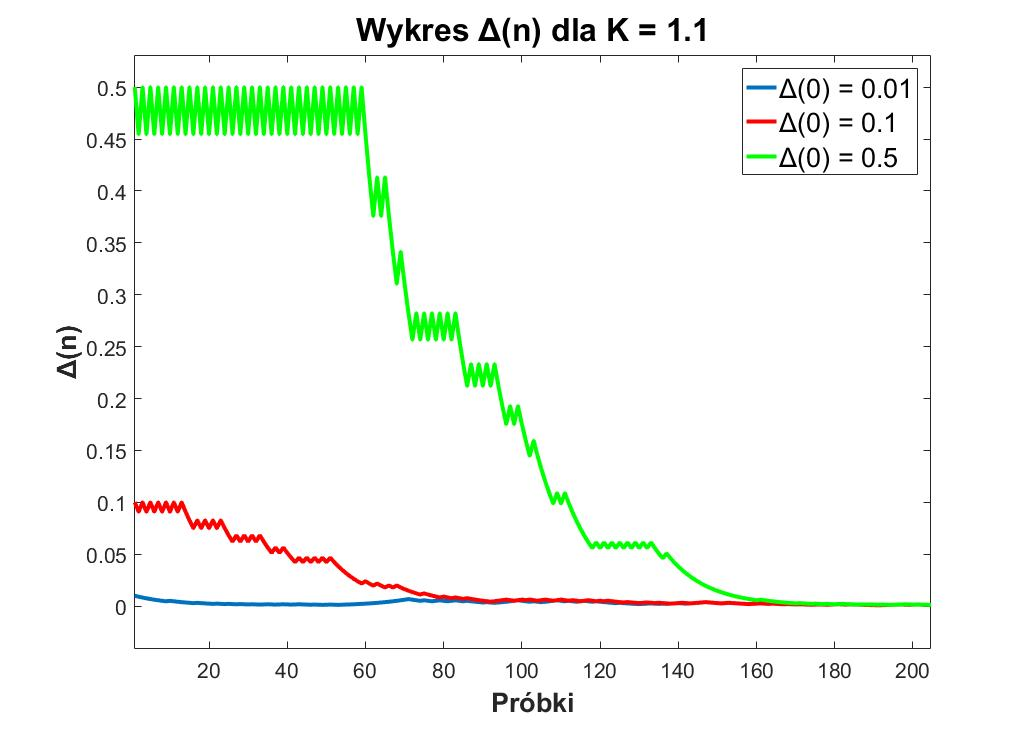
\includegraphics[scale=0.33]{f2.jpg}
\end{figure}
\begin{center}
Okres przejściowy T$_p$ = 160 próbek
\end{center}
\clearpage
\begin{figure}[h]
\centering
\caption{Wykres $\Delta$(n) dla K = 1.5}
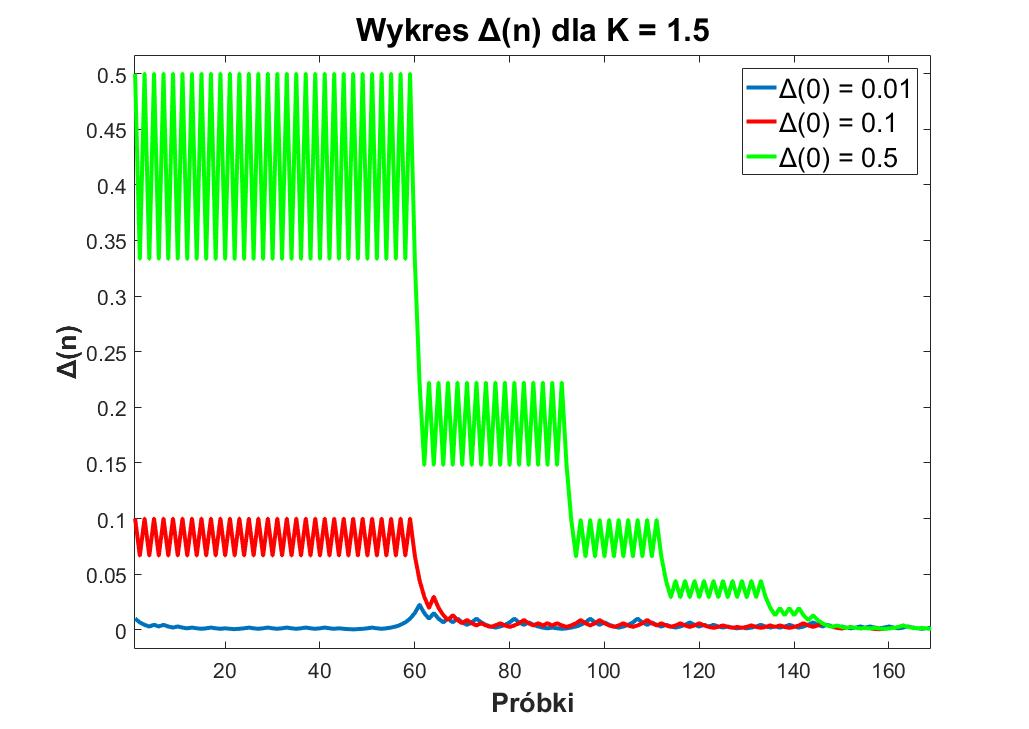
\includegraphics[scale=0.33]{f3.jpg}
\end{figure}
\begin{center}
Okres przejściowy T$_p$ = 145 próbek
\end{center}
\begin{figure}[h]
\centering
\caption{Wykres $\Delta$(n) dla K = 2.0}
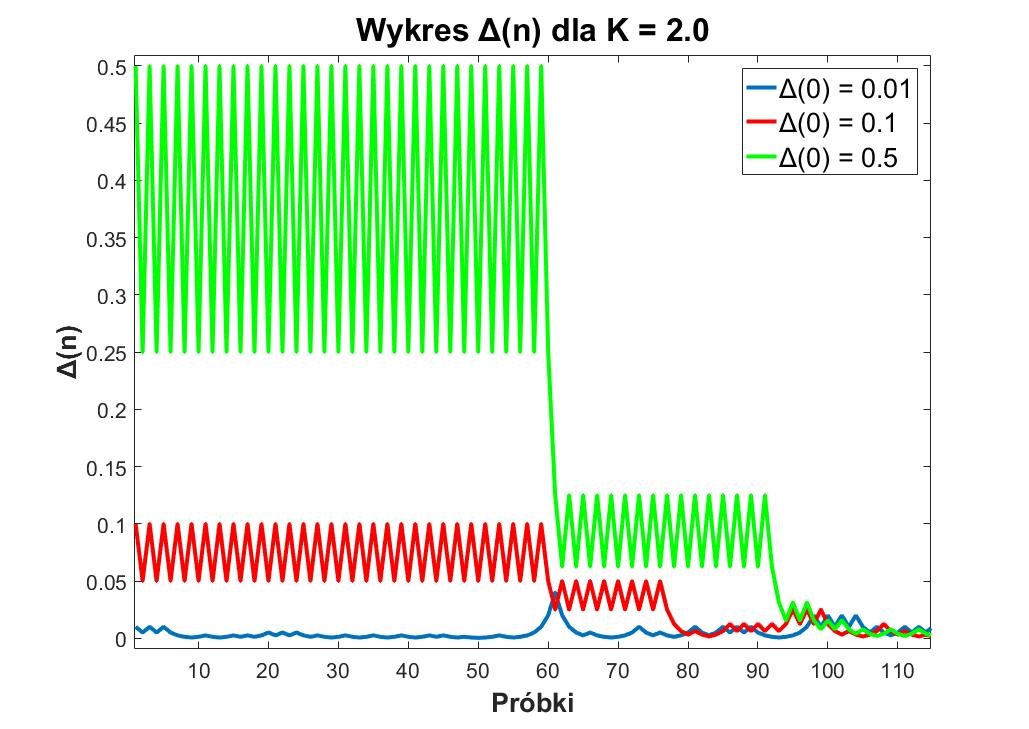
\includegraphics[scale=0.33]{f4.jpg}
\end{figure}
\begin{center}
Okres przejściowy T$_p$ = 100 próbek
\end{center}
\indent\indent Z powyższych wykresów wprost wynika, że wraz ze wzrostem wartości K maleje okres przejściowy. Jednak dla dowolnej wartości parametru K, jeśli przyjąć $\Delta$(0) = 0.01  to okres przejściowy T$_p$ = 0. Do dalszych obliczeń (po wyznaczeniu obszaru pracy) przyjęta zostanie $\Delta$(0) = 0.01.
\clearpage
\subsection{Wyznaczanie obszaru pracy}
\begin{figure}[h]
\centering
\caption{Wykres $\Delta$(n) dla K = 1.01}
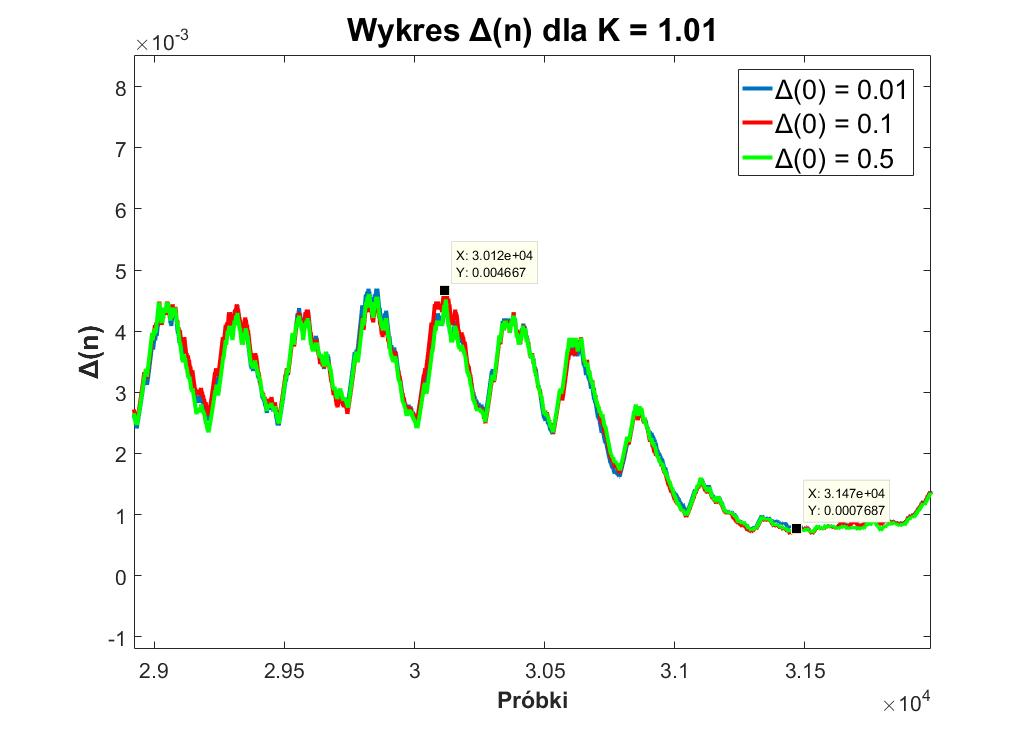
\includegraphics[scale=0.33]{f5.jpg}
\end{figure}
\begin{center}
Obszar pracy $\Delta$(n) = 4.70 $\cdot$ 10$^{-3}$ - 0.76 $\cdot$ 10$^{-3}$ = 3.94 $\cdot$ 10$^{-3}$
\end{center}
\begin{figure}[h]
\centering
\caption{Wykres $\Delta$(n) dla K = 1.1}
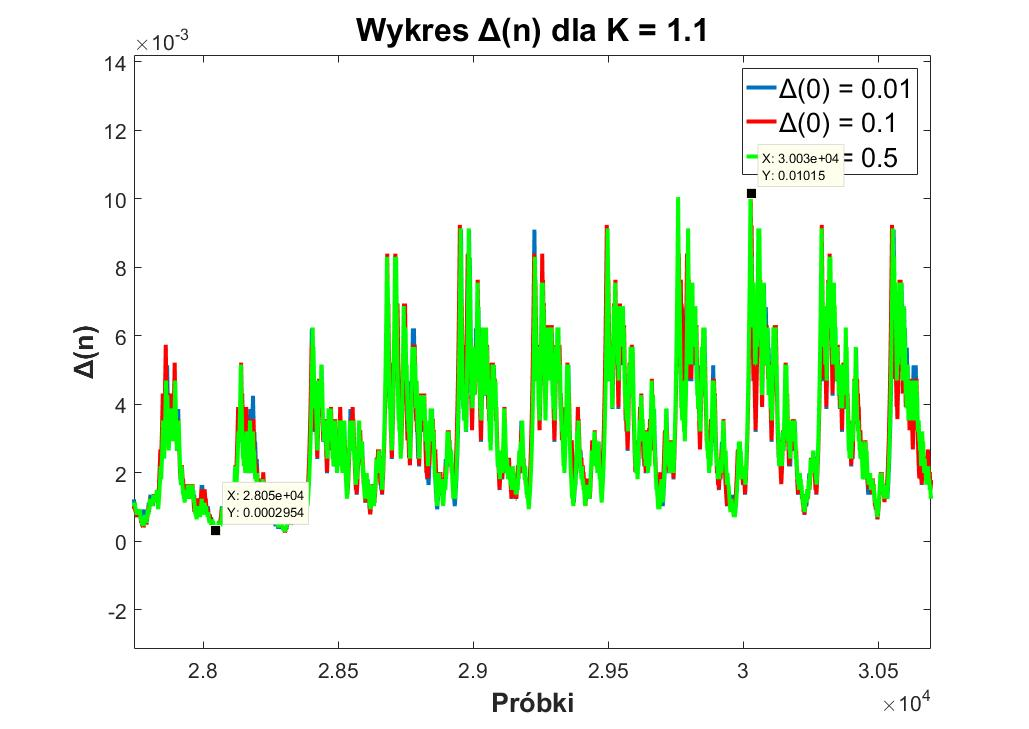
\includegraphics[scale=0.33]{f6.jpg}
\end{figure}
\begin{center}
Obszar pracy $\Delta$(n) = 10.15 $\cdot$ 10$^{-3}$ - 0.29 $\cdot$ 10$^{-3}$ = 9.86 $\cdot$ 10$^{-3}$
\end{center}
\clearpage
\begin{figure}[h]
\centering
\caption{Wykres $\Delta$(n) dla K = 1.5}
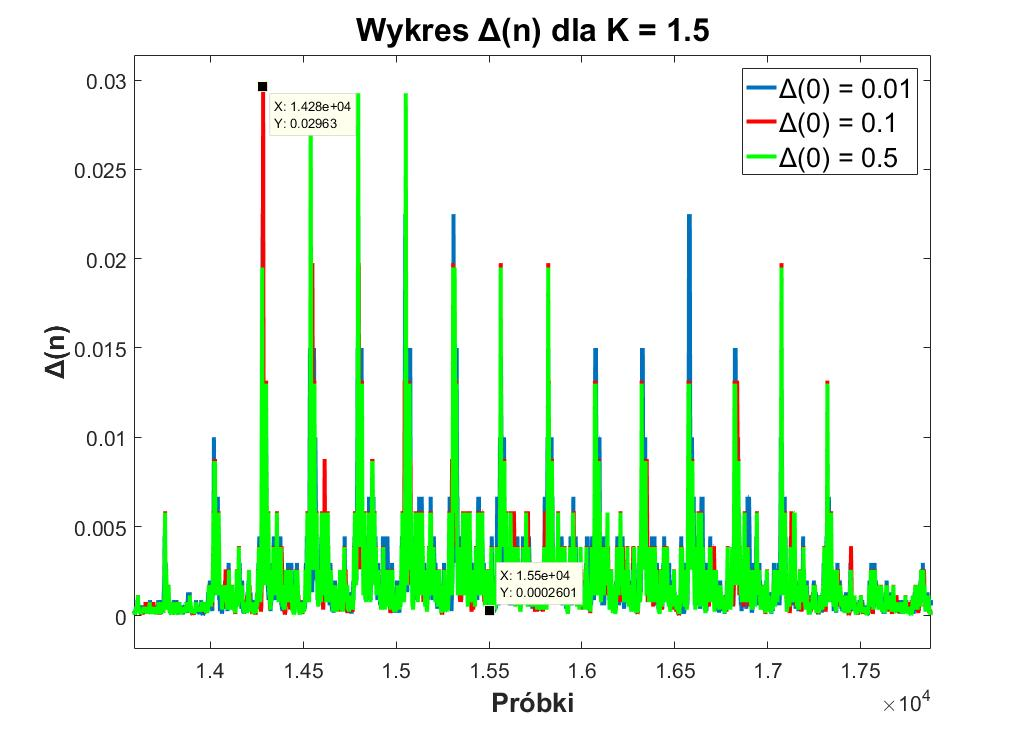
\includegraphics[scale=0.33]{f7.jpg}
\end{figure}
\begin{center}
Obszar pracy $\Delta$(n) = 29.63 $\cdot$ 10$^{-3}$ - 0.20 $\cdot$ 10$^{-3}$ = 29.43 $\cdot$ 10$^{-3}$
\end{center}
\begin{figure}[h]
\centering
\caption{Wykres $\Delta$(n) dla K = 2.0}
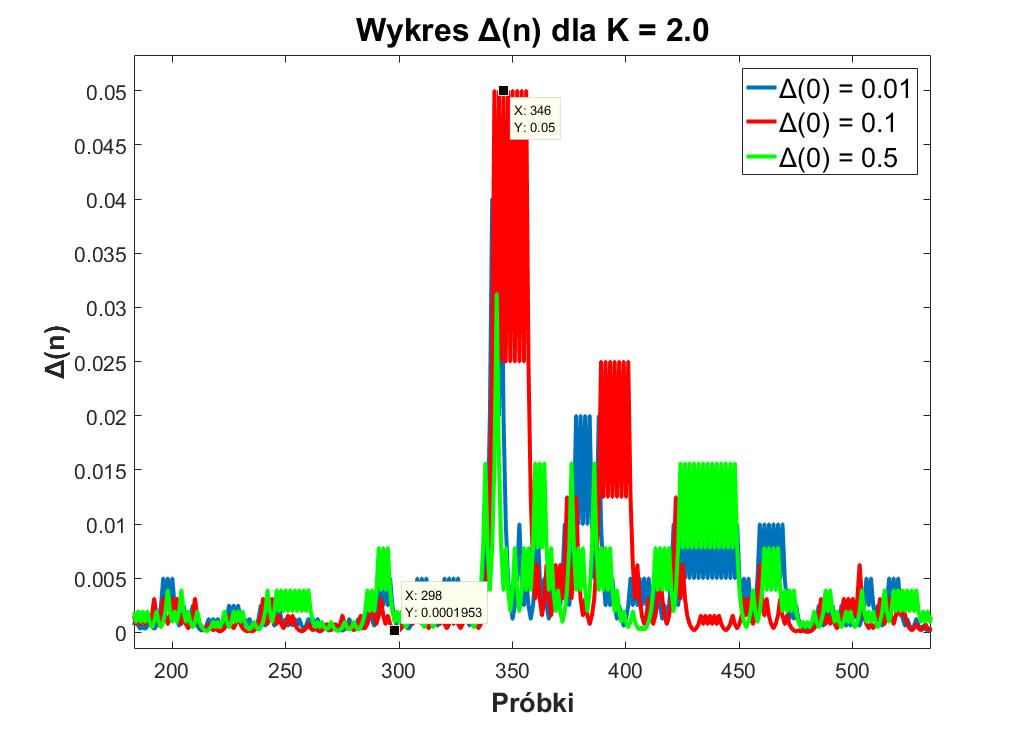
\includegraphics[scale=0.33]{f8.jpg}
\end{figure}
\begin{center}
Obszar pracy $\Delta$(n) = 50.00 $\cdot$ 10$^{-3}$ - 0.19 $\cdot$ 10$^{-3}$ = 49.81 $\cdot$ 10$^{-3}$
\end{center}
\indent\indent Z wykresów na rys. 6 - 9 możemy wyznaczyć obszar pracy. Jak widać dla K $\leq$ 1.5 obszar pracy rozszerza się w górę i w dół. Dla K = 2.0 obszar pracy rośnie jedynie w górę. Dla K $\geq$ 1.5 pojawia się też szum śrutowy i staje się on bardzo silny już dla K = 2 (obserowany na rys. 9 nieustannie). Przyjmujemy więc obszar poszukiwań K w zakresie (1; 2].
\clearpage
\subsection{Wyznaczanie optymalnej wartości K}
\begin{figure}[h]
\centering
\caption{Wykres SQNR = f(K), $\Delta$(0) = 0.01}
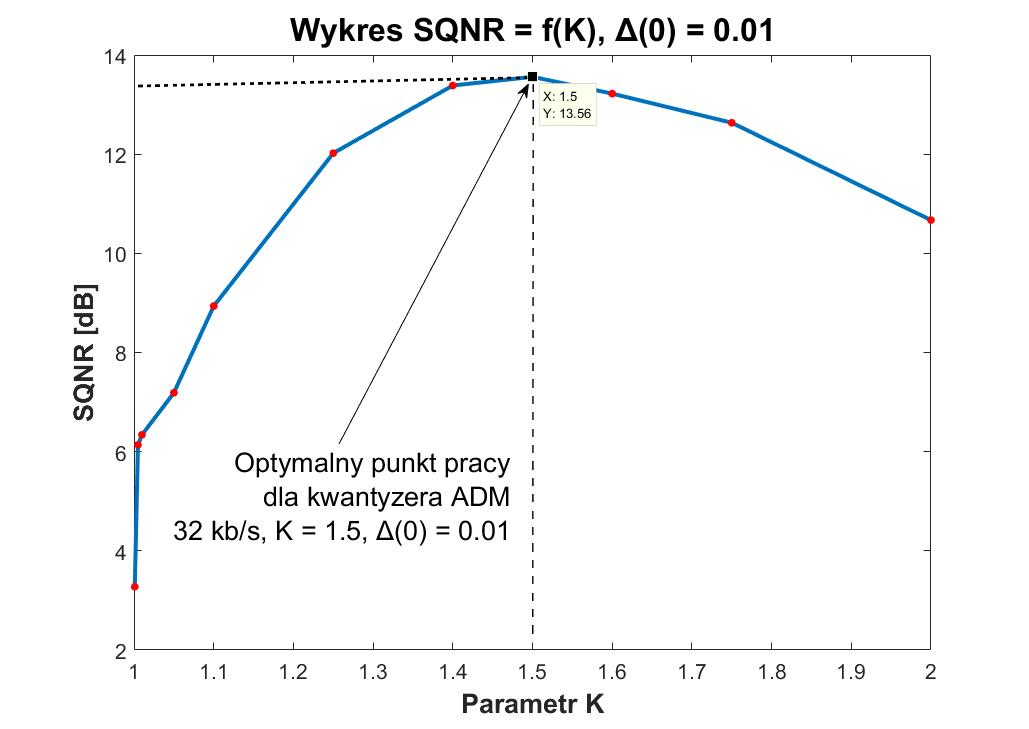
\includegraphics[scale=0.33]{f9.jpg}
\end{figure}
\begin{figure}[h]
\centering
\caption{Porównanie sygnału oryginalnego z sygnałem modulowanym}
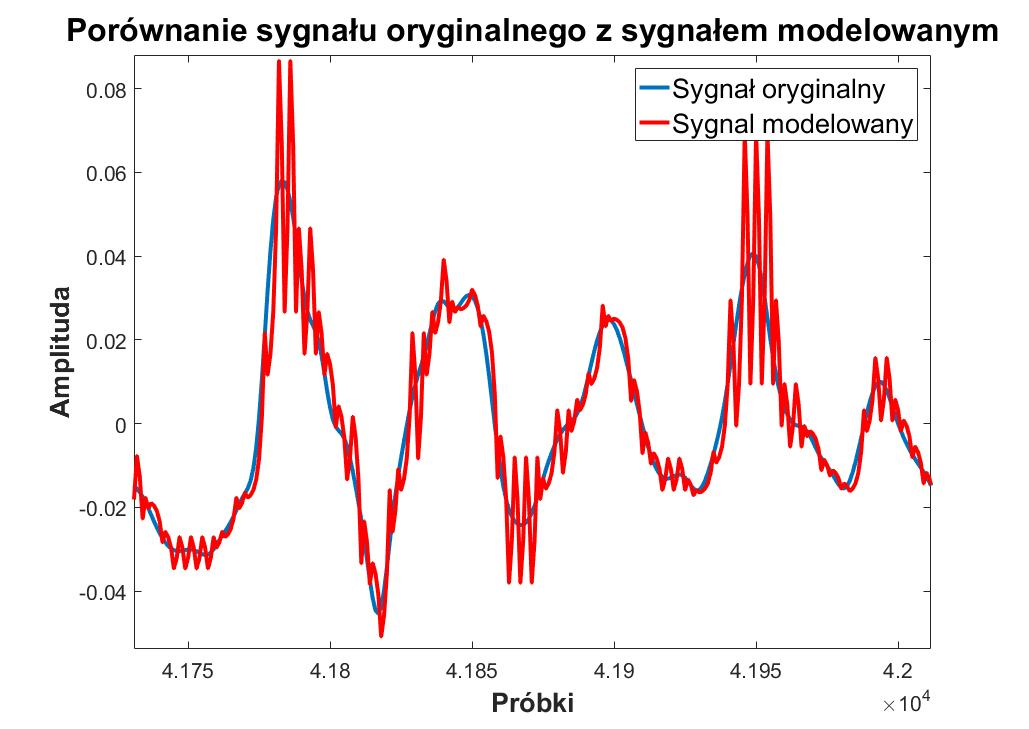
\includegraphics[scale=0.33]{f10.jpg}
\end{figure}
\indent\indent Dla wartości K = 1.5 otrzymujemy najlepszy SQNR. Funkcja SQNR = f(K) osiąga wtedy maksimum i przyjmuje wartość f(1.5) = 13.56 dB. Na rys. 11 widzimy, że w otoczeniu lokalnych maksimów funkcji oryginalnej występuje lekki szum śrutowy, jednak jak wskazuje SQNR jest on optymalny względem jakości sygnału.
\clearpage
\subsection{Wyznaczanie optymalnej długości filtru adaptacyjnego}
\begin{figure}[h]
\centering
\caption{Wykres SQNR = f(p)}
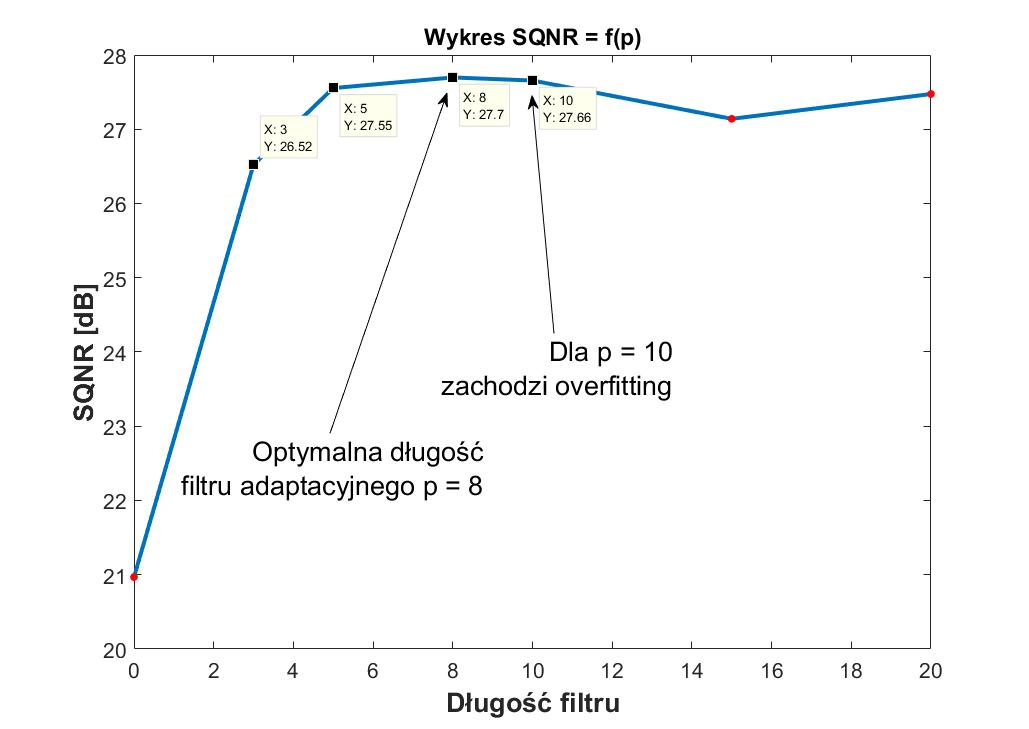
\includegraphics[scale=0.33]{f11.jpg}
\end{figure}
\subsection{Tabele podsumowujące odczytane z wykresów własności}
% Table generated by Excel2LaTeX from sheet 'Arkusz1'
\begin{table}[h]
  \centering
  \caption{Podsumowanie okresu przejściowego, obszaru pracy oraz uwagi dla zmiennego K}
    \begin{tabular}{|c|c|c|c|}\hline
    $K$ & $T_p$ & $\Delta(n)~\cdot 10^{-3}$ & Uwagi \\\hline
    1.01 & 600 & 3.94 & dla $\Delta$(0) = 0.01 brak stanu przejściowego \\\hline
    1.1 & 160 & 9.86 & dla $\Delta$(0) = 0.01 brak stanu przejściowego \\\hline
    1.5 & 145 & 29.43 & dla $\Delta$(0) = 0.01 brak stanu przejściowego, efekt szumu śrutowego \\\hline
    2 & 100 & 49.81 & dla $\Delta$(0) = 0.01 brak stanu przejściowego, nieustanny szum śrutowy \\\hline
    \end{tabular}%
  \label{tab:addlabel}%
\end{table}%
% Table generated by Excel2LaTeX from sheet 'Arkusz1'
\begin{table}[h]
  \centering
  \caption{Wartość SQNR, zmiana SQNR, ilość elementarnych mnożeń (K) oraz ilość mnożeń w~ciągu 1 sekundy (R) w zależności od długości filtru (p)}
    \begin{tabular}{|c|c|c|c|c|}\hline
    $P$ & $SQNR~[dB]$ & $\Delta SQNR~[dB]$ & $K$ & $R$ \\\hline
    0 & 21 & 0 & 1 & 8000 \\\hline
    3 & 26.52 & 5.52 & 10 & 80000 \\\hline
    5 & 27.58 & 1.06 & 16 & 128000 \\\hline
    8 & 27.75 & 0.17 & 25 & 200000 \\\hline
    \end{tabular}%
  \label{tab:addlabel}%
\end{table}%
\clearpage
\section{Wnioski}
\subsection{ADM}
\begin{itemize}
\item Pętla sprzężenia zwrotnego uzależniona jest od wartości parametru K. W miarę wzrostu K~maleje czas okresu przejściowego.
\item Zwiększając K do wartości 1.5, obserwujemy zwiększenie obszaru pracy zarówno w dół, jak i~w~górę. Dla wartości K = 2 obserwujemy jedynie wzrost obszaru pracy w górę.
\item Przyjmując dowolne z badanych K, obserwujemy że dla $\Delta$(0) = 0.01 nie ma stanu przejściowego, co jest pożądanym efektem.
\item Wyznaczona optymalna wartość K = 1.5 (dla $\Delta$(0) = 0.01). Dla tych parametrów osiągamy najwyższą wartość SQNR = 13.56 dB.
\item Dla K = 1.5 zaobserwowano szum śrutowy w okolicach lokalnych maksimów funkcji oryginalnej, jednak jak pokazano jest to optymalna wartość parametru K w sensie SQNR.
\end{itemize}
\subsection{ADPCM}
\begin{itemize}
\item Optymalna długość filtru p = 8 w sensie SQNR.
\item Warto również wziąć pod uwagę (jednak nie jest to element wykonanego ćwiczenia) p = 3, a~także p = 5. Pomiędzy p = 3, a p = 8 obserwujemy $\Delta$SQNR = 1.23 dB, a pomiędzy p~=~5 i~p~=~8 obserwujemy jedynie $\Delta$SQNR = 0.17 dB. Są to wartości na tyle małe, że przy mniejszych zasobach sprzętowych można byłoby bez zauważalnej utraty jakości skrócić filtr do tych wartości.
\item Warte rozważenia jest także przyjęcie funkcji kosztu zależnej nie tylko od SQNR, ale także od ilości mnożeń wykonywanych w ciągu sekundy: V(SQNR, R) = SQNR $\pm$ $\gamma\cdot$R.
\item Do realizacji kodera ADPCM potrzebna jest szybkość transmisji 32 kb/s, ponieważ każda próbka reprezentowana jest przez 4 bity. Pobieramy 8 000 próbek na sekundę (częstotliwość próbkowania 8 kHz), więc: 4 bity $\cdot$ 8000 $\frac{1}{s}$ = 32 000 $\frac{b}{s}$ = 32 $\frac{kb}{s}$.
\end{itemize}
\clearpage
\section{Literatura}
[1] Materiały udostępnione do wykładu dr. inż. Roberta Hossy.
\end{document}